\chapter{Other SUSY results}
\label{chap:summary_susy}

In this chapter we discuss the interplay of the searched presented in the previous two chapters and the 
wide program of \gls{susy} searched carried on by the \gls{atlas} and \gls{cms} collaborations. 

\section{Gluino pair production}

\begin{figure}[htbp]
	\centering
	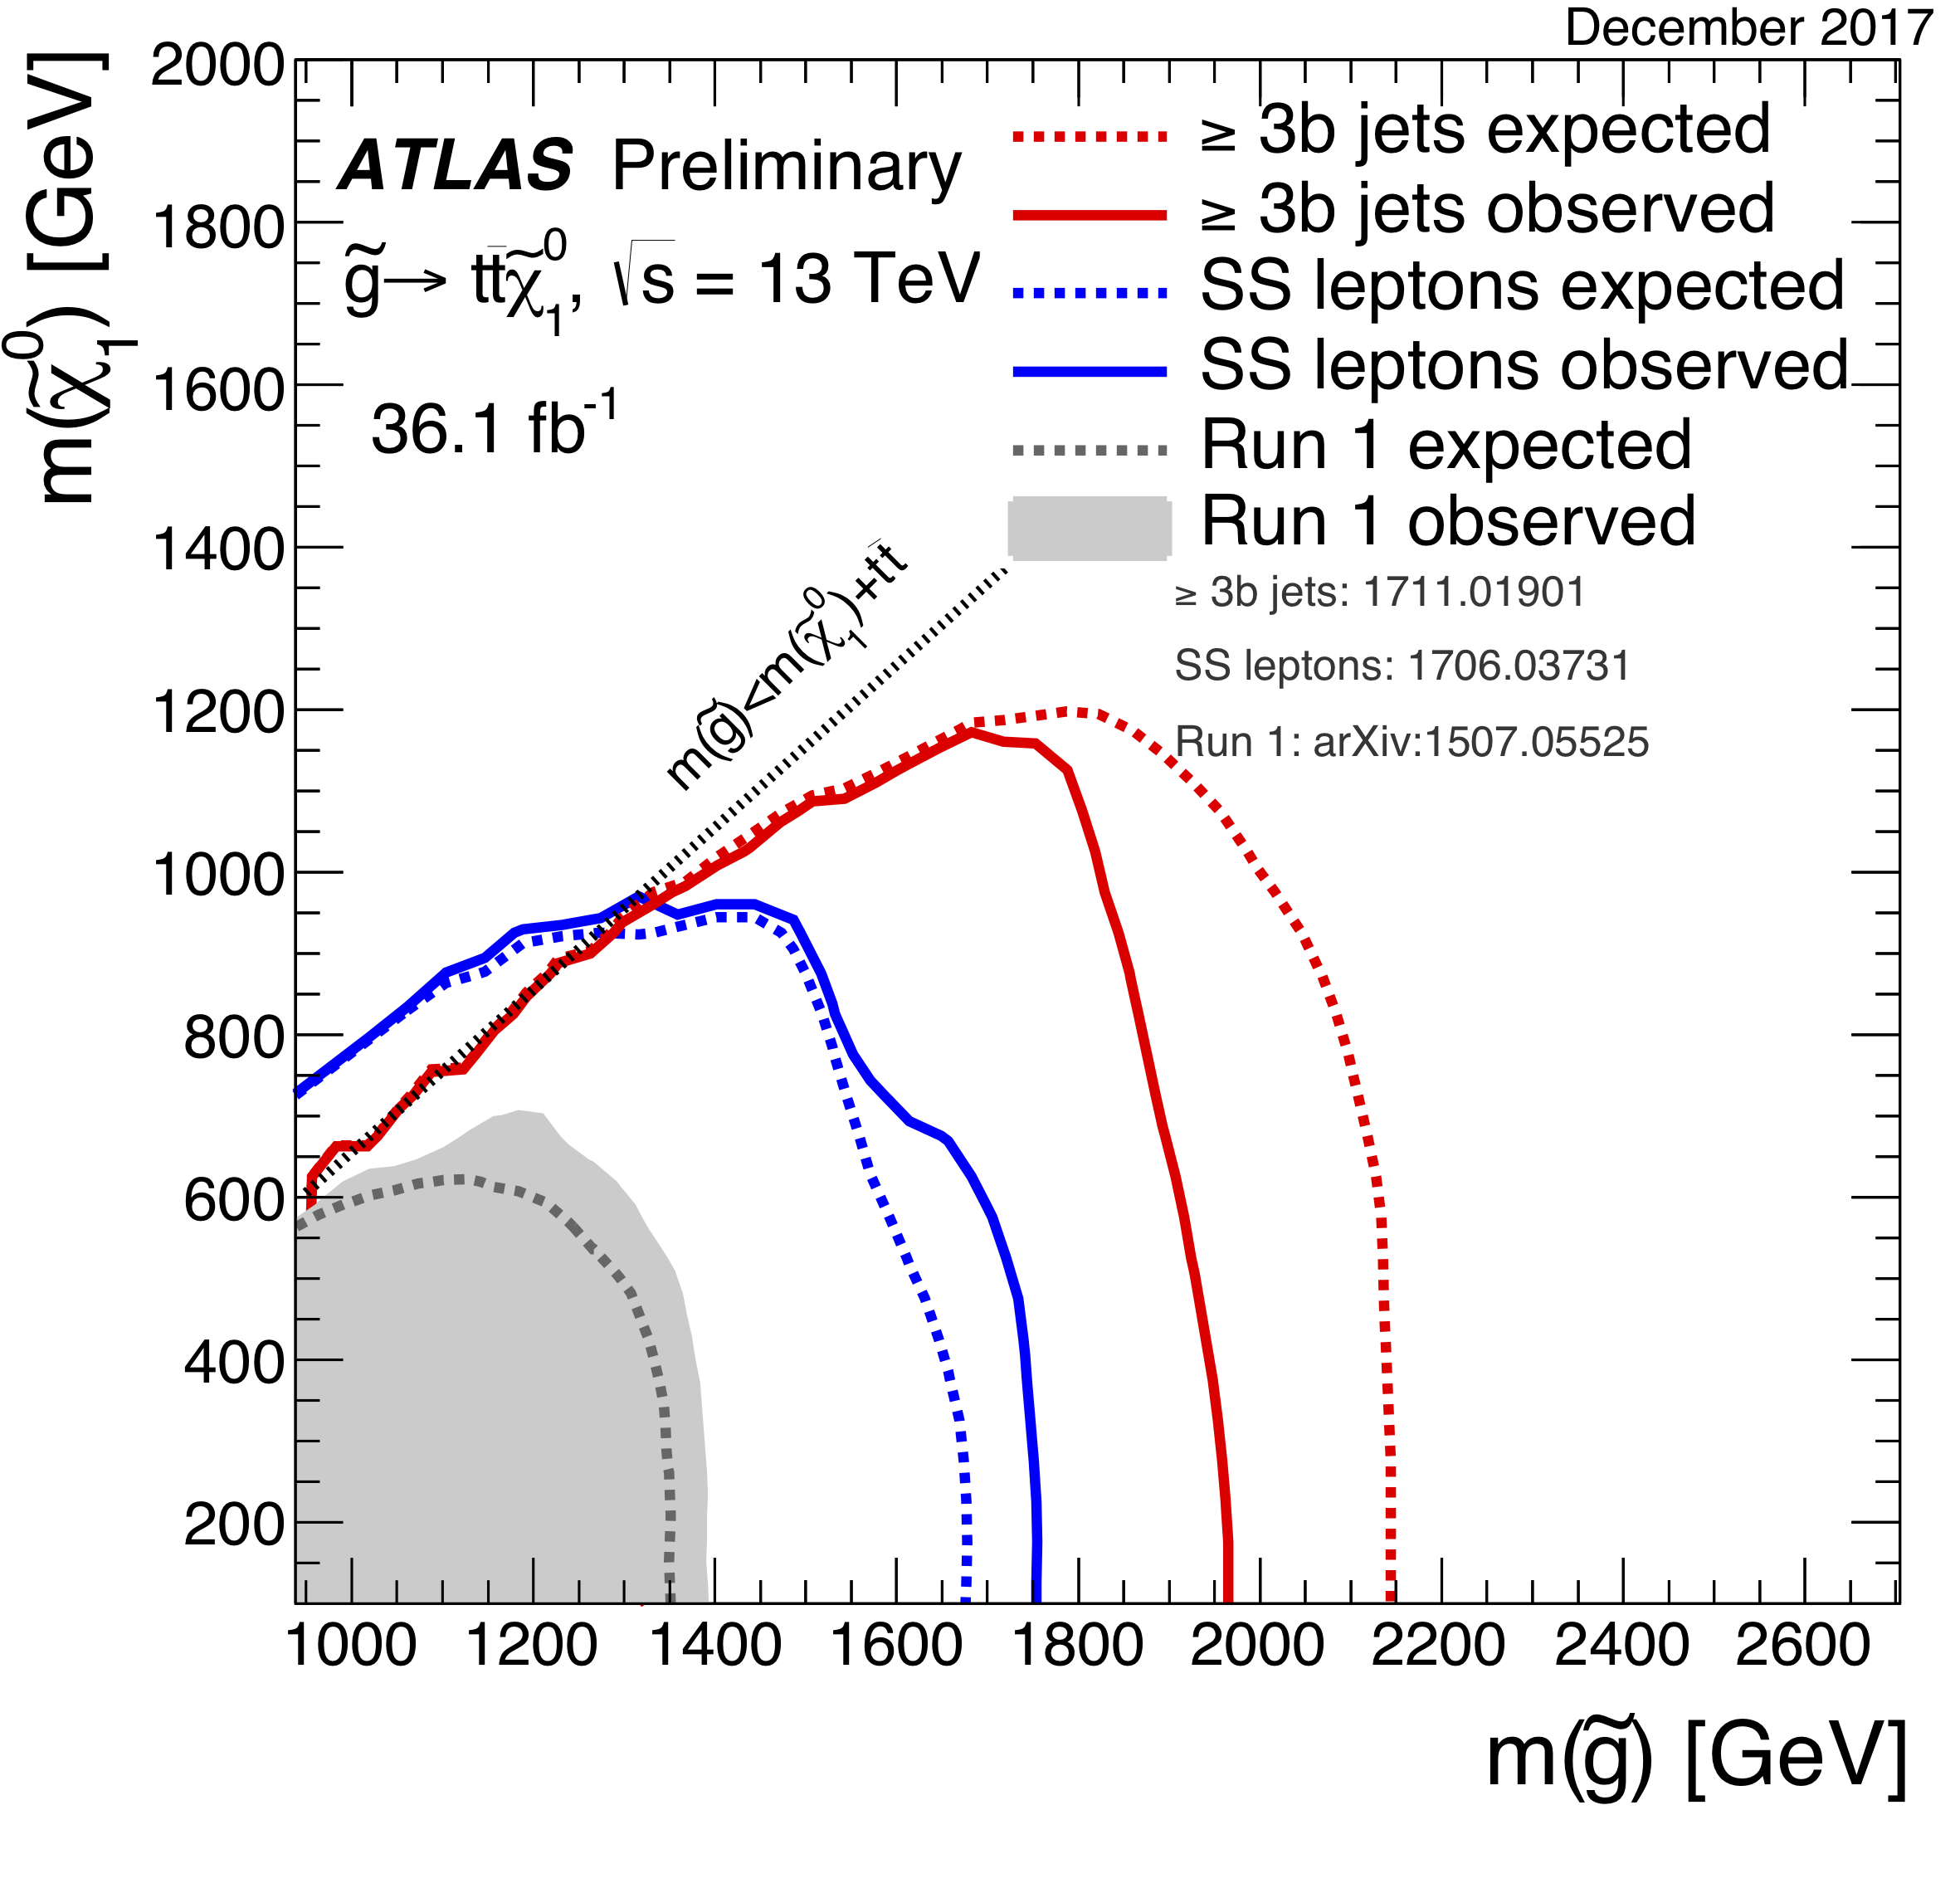
\includegraphics[width=0.65\textwidth]{figures/summary_plots/ATLAS_SUSY_Gtt}
	\caption{Exclusion limits at 95\% CL based on 13 TeV data in the (gluino, lightest neutralino) 
	mass plane for the Gtt simplified model where a pair of gluinos decays promptly via off-shell top 
	squarks to four top quarks and two lightest neutralinos. Theoretical signal cross section uncertainties are 
	not included in the limits shown. 
	} 
	\label{fig:summary_atlas_Gtt}
\end{figure}

\section{RPV interpretation}

\FloatBarrier

\section{Higgsino pair production in GMSB models}

\begin{figure}[htbp]
	\centering
	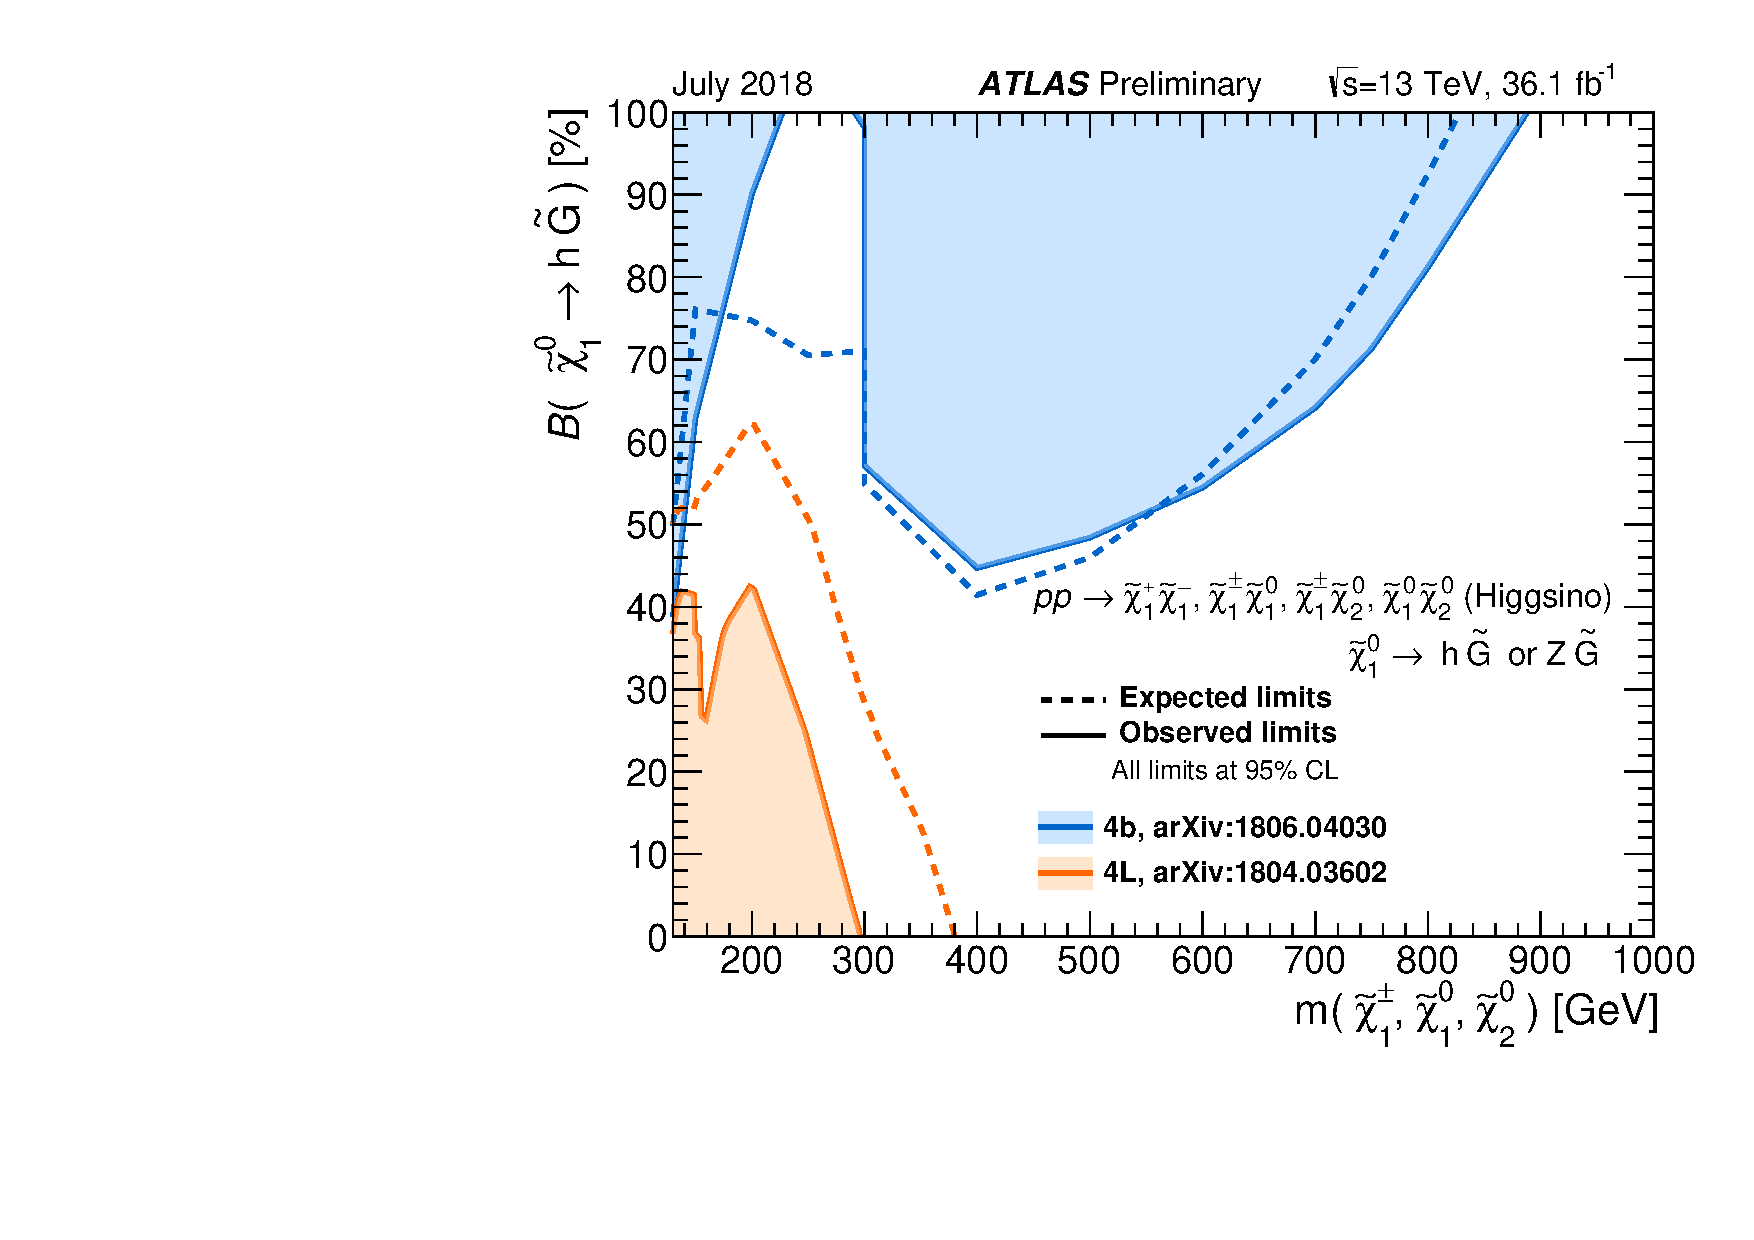
\includegraphics[width=0.65\textwidth]{figures/summary_plots/ATLAS_SUSY_EWSummary_GGM.pdf}
	\caption{The 95\% CL exclusion limits on a general gauge mediation model from 13 TeV data. 
	The model assumes a pure Higgsino NLSP that promptly decays to either Z gravitino or Higgs gravitino. 
	The limits are displayed as a function of the mass of the nearly mass-degenerate Higgsino triplet and the branching fraction of lightest Higgsino to Higgs gravitino. 	
	} 
	\label{fig:summary_atlas_higgsino_GMSB}
\end{figure}

\FloatBarrier


\begin{figure}[htbp]
	\centering
	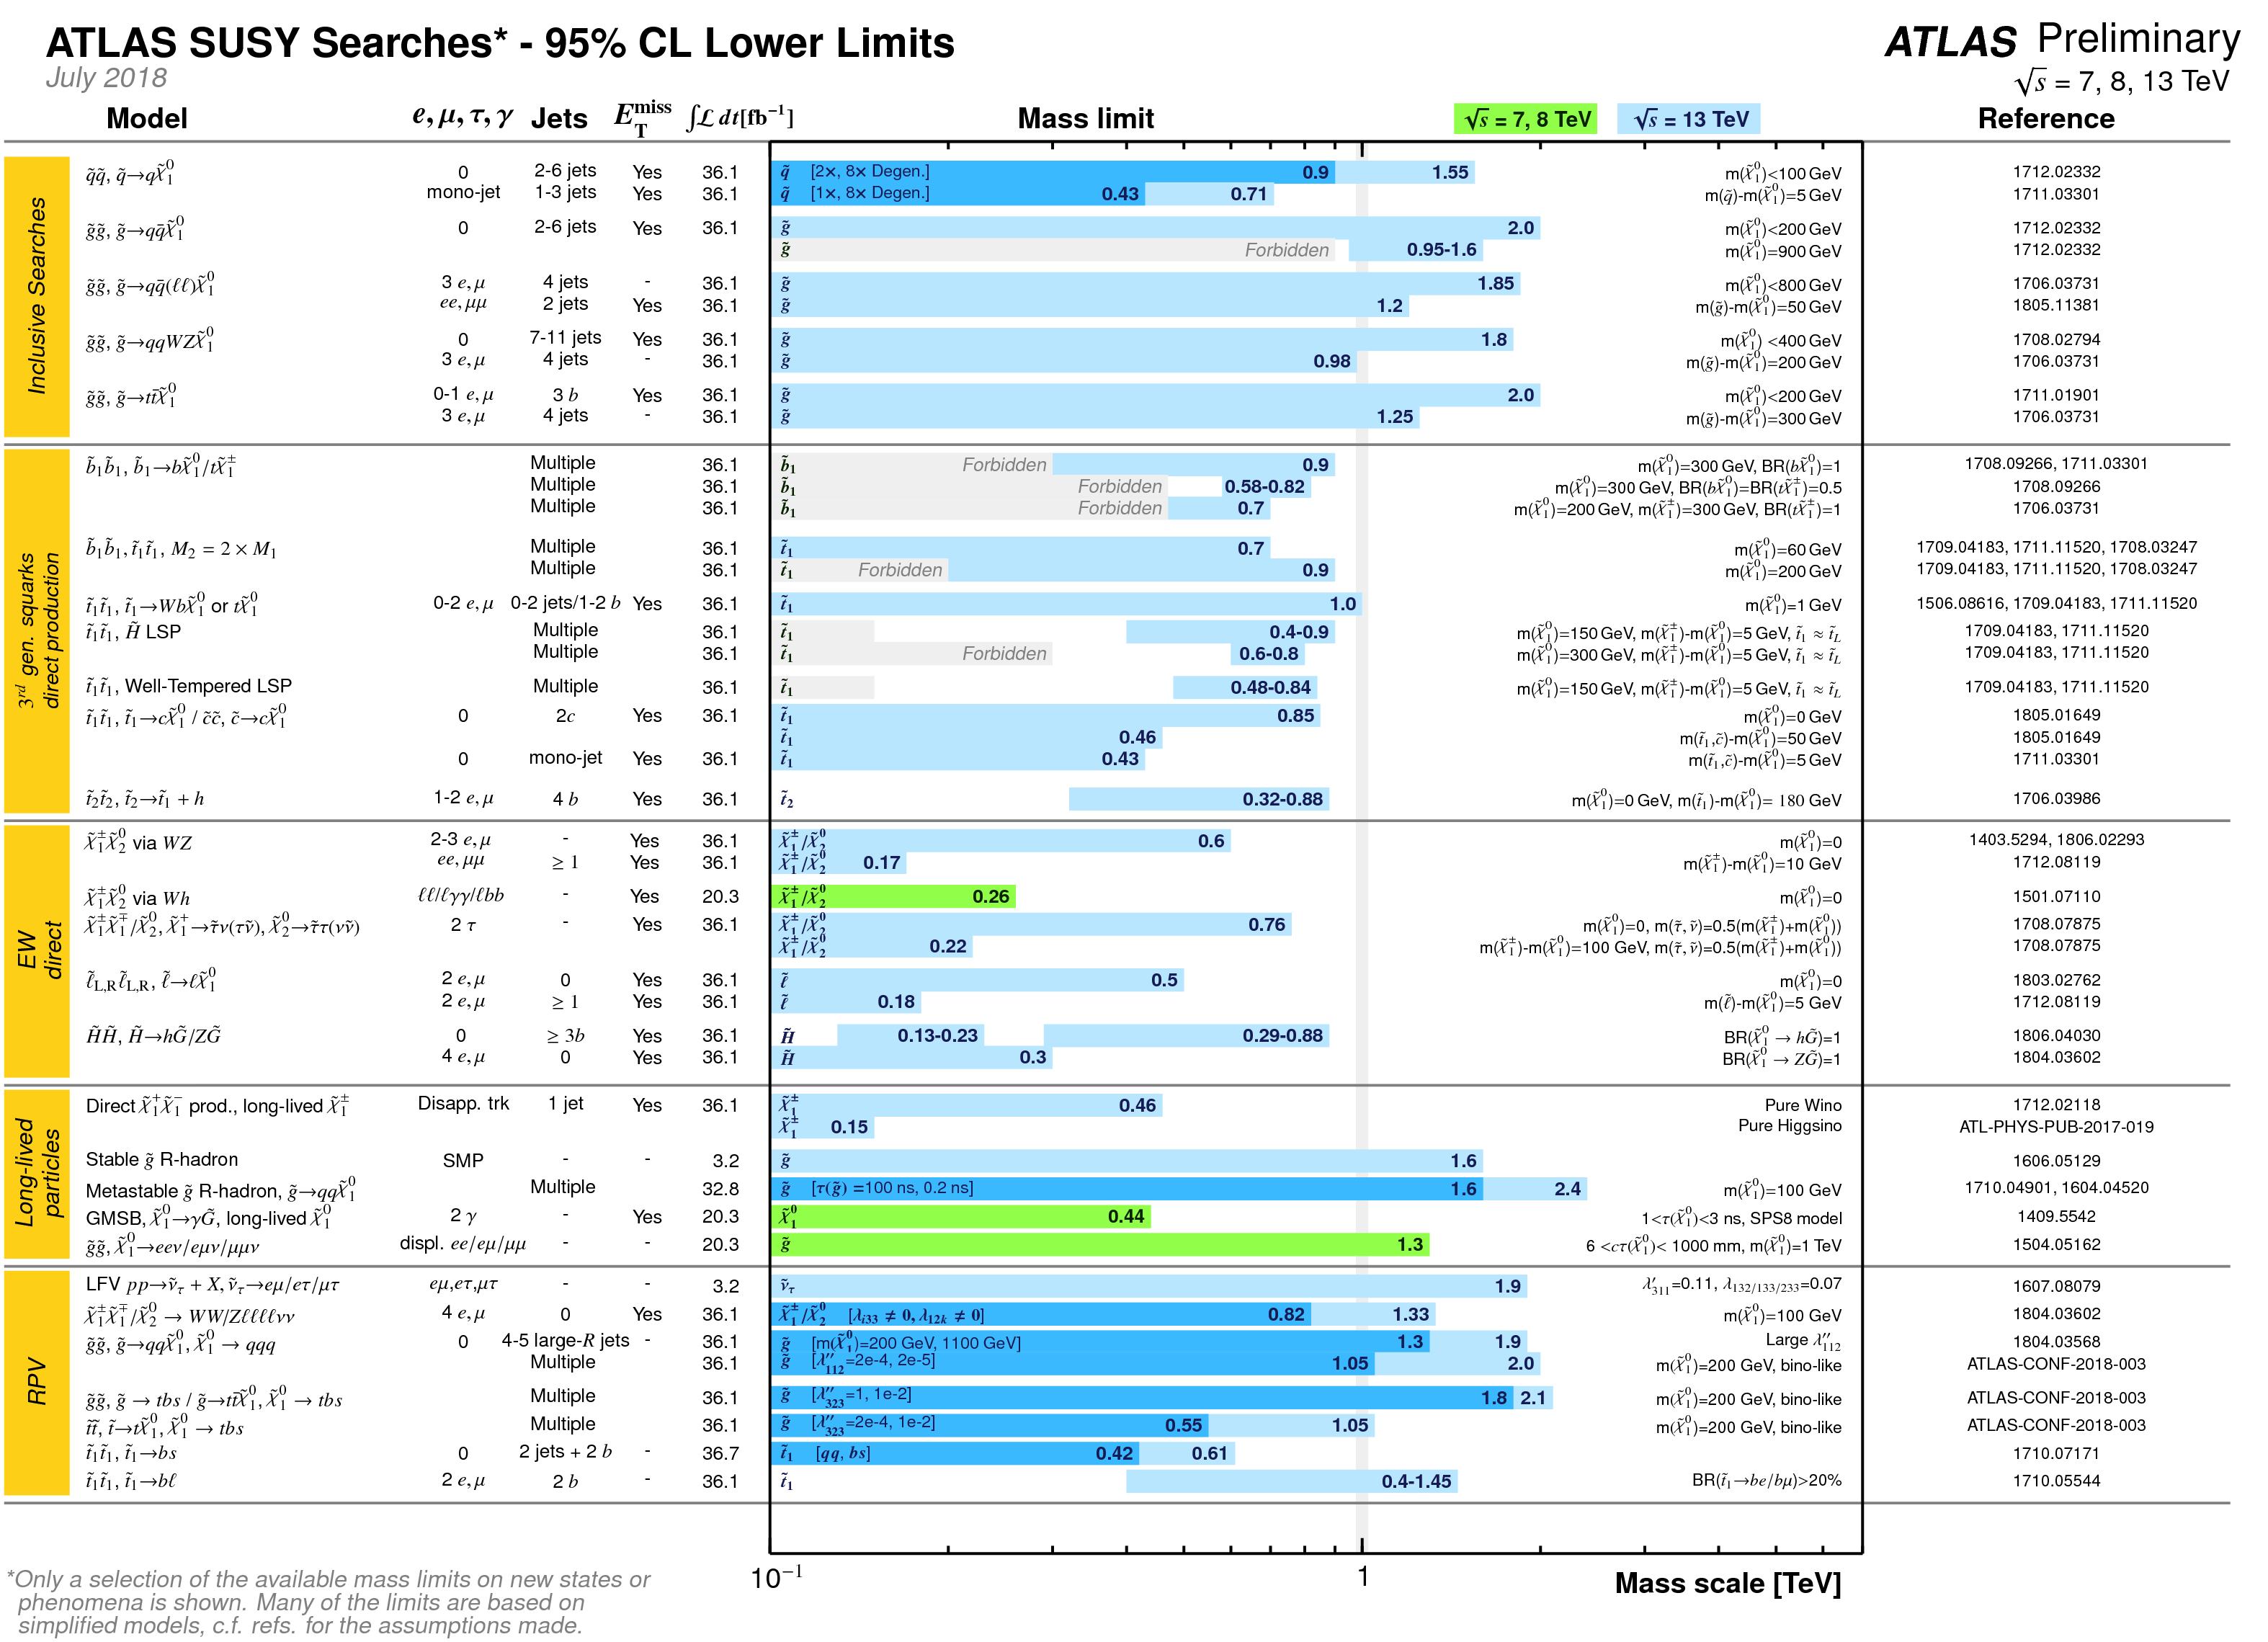
\includegraphics[width=1\textwidth]{figures/summary_plots/ATLAS_SUSY_Summary.png}
	\caption{	Mass reach of the ATLAS searches for Supersymmetry. 
	A representative selection of the available search results is shown. Results are quoted for the nominal cross section 
	in both a region of near-maximal mass reach and a demonstrative alternative scenario, in order to display the range in 
	model space of search sensitivity. Some limits depend on additional assumptions on the mass of the intermediate states, 
	as described in the references provided in the plot. 
	} 
	\label{fig:summary_atlas_summary}
\end{figure}